\section{Radiation pressure modeling for LRO}

\subsection{Lunar albedo radiation}
\label{subsec:lunar-albedo}

\begin{figure*}[t]
    \centering

    \begin{subfigure}[c]{0.49\textwidth}
        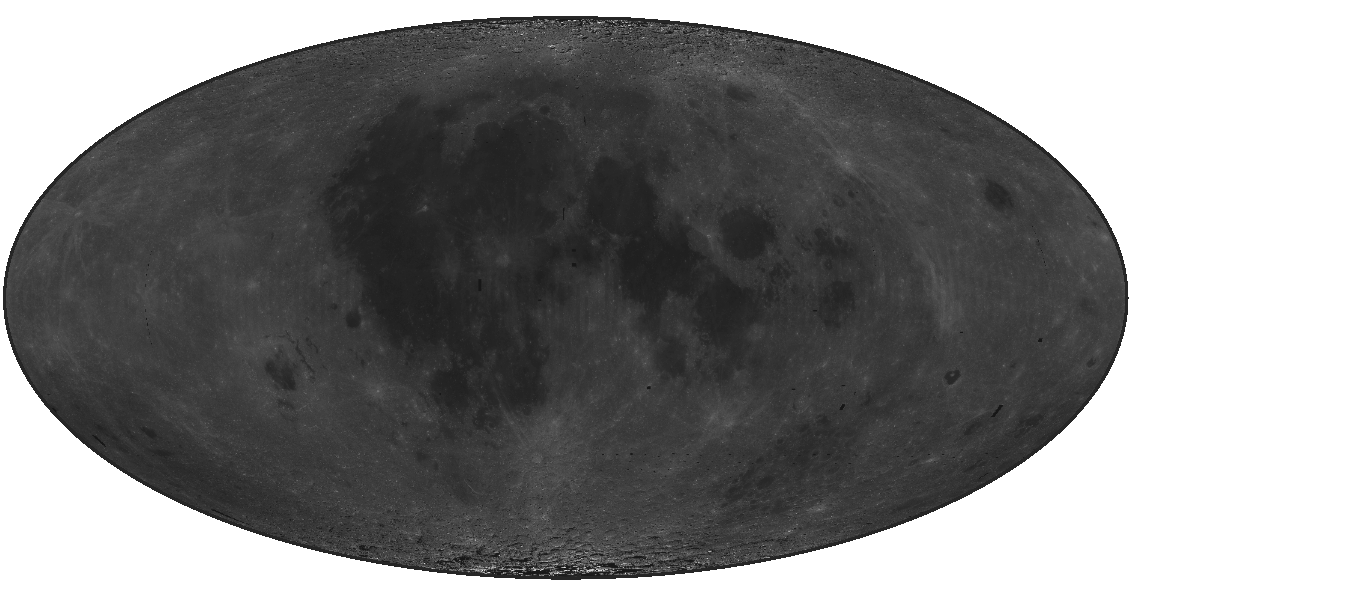
\includegraphics[width=\textwidth]{figures/plots/lunar_map_photo.pdf}
        \subcaption{}
        \label{fig:lunar-albedo-map-photo}
    \end{subfigure}
    \hfill
    \begin{subfigure}[c]{0.49\textwidth}
        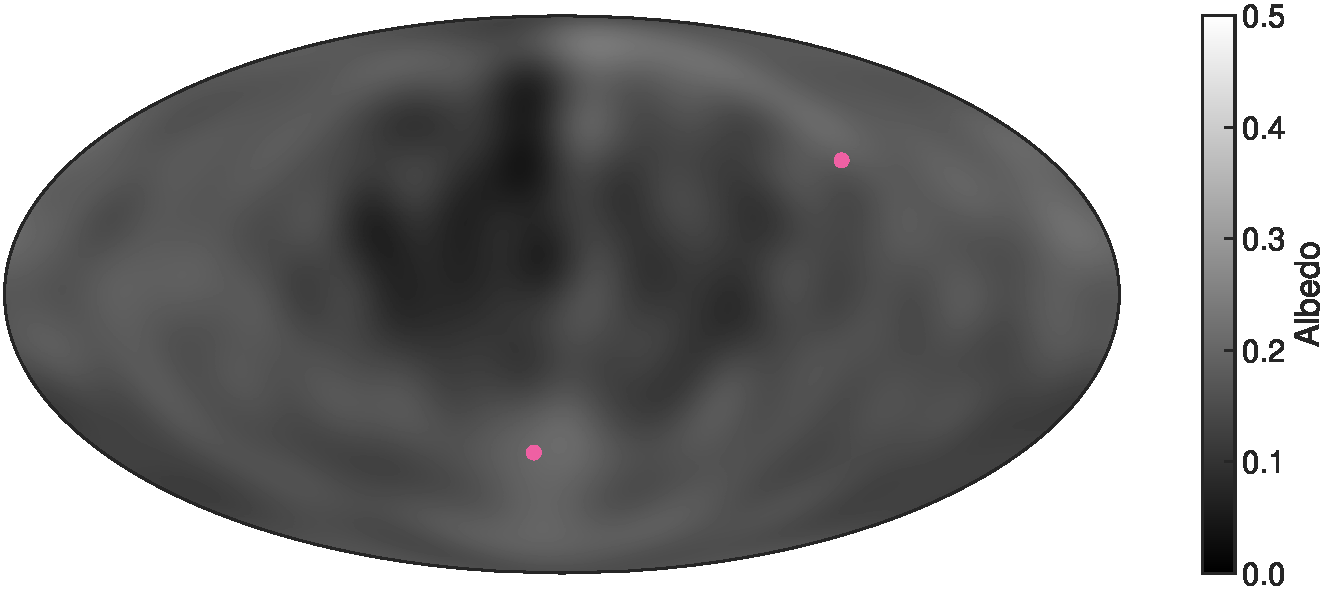
\includegraphics[width=\textwidth]{figures/plots/lunar_map_dlam1.pdf}
        \subcaption{}
        \label{fig:lunar-albedo-map-dlam1}
    \end{subfigure}

    \bigskip

    \begin{subfigure}[c]{0.49\textwidth}
        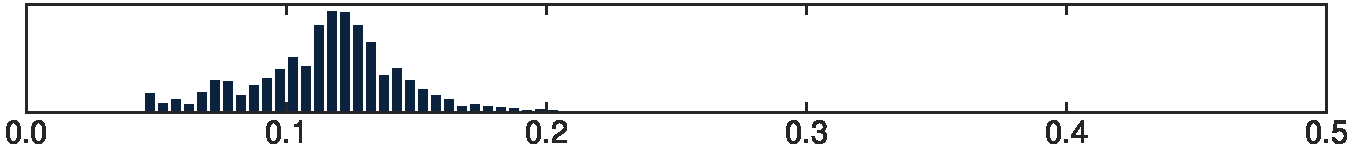
\includegraphics[width=\textwidth]{figures/plots/lunar_hist_photo.pdf}
        \subcaption{Mosaic (mean = 0.12, minimum = 0.05, 99th percentile = 0.29)~\cite{UASC2009}}
    \end{subfigure}
   \hfill
    \begin{subfigure}[c]{0.49\textwidth}
        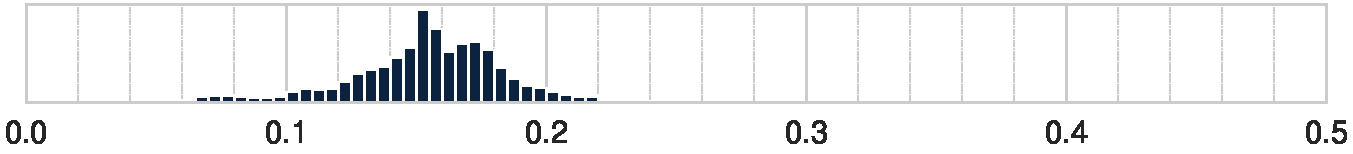
\includegraphics[width=\textwidth]{figures/plots/lunar_hist_dlam1.pdf}
        \subcaption{\acrshort{DLAM1} (mean = 0.15, minimum = 0.04, 99th percentile = 0.22)}
    \end{subfigure}

   \caption{Lunar albedo distribution from Clementine. Both the mosaic and \acrshort{DLAM1} are based on 750 nm reflectivity, but \acrshort{DLAM1} has been corrected to the average solar wavelength. Bright features like the Tycho and Giordano Bruno craters (\textcolor{mpl-pink}{\ding{108}}) can be registered. Note that the maximum of the albedo scales is 0.5 to increase contrast; in reality, the Moon appears half as bright.}
   \label{fig:lunar-albedo-map}
\end{figure*}

The Moon is a major source of radiation in \gls{LRO}'s orbit, with lunar irradiance magnitudes approaching half of the Sun's. Therefore, albedo and thermal radiation due to the Moon will be modeled. While lunar albedo is only \qty{40}{\percent} of Earth's albedo~\cite{Goode2001}, albedo radiation is still substantial, particularly over the subsolar point~\cite{Floberghagen1999}. However, lunar albedo varies significantly with geology: the highlands (mean $a = 0.16$, maximum $a=0.25$) are much more reflective than the maria (mean $a = 0.07$, minimum $a = 0.05$) due to their respective regolith composition~\cite{Vasavada2012,Hayne2017,Sato2014}. The mosaic of calibrated albedo imagery from Clementine in \cref{fig:lunar-albedo-map-photo} clearly shows the differences between highlands and marias. The mean of 0.12 agrees with other literature~\cite{Vasavada2012}, and most of the lunar surface has an albedo below 0.20. Higher values are only found at the poles, where the imagery represents topographic shading rather than actual albedo~\cite{McEwen1997}. Note that the mosaic is for albedo of light at \qty{750}{\nm} wavelength, which is slightly longer than the average solar wavelength. Even though solar radiation has most energy within the \qtyrange{300}{2400}{\nm} band, the spectrum peaks at around \qty{470}{\nm}. Lunar reflectivity increases with increasing wavelength~\cite{Shkuratov2011}.

\citeauthor{Floberghagen1999}'s \numproduct{15x15} spherical harmonics expansion called \gls{DLAM1}~\cite{Floberghagen1999} is often used to represent this spatial albedo variability in lunar \gls{RP} models. \gls{DLAM1} was fitted from Clementine imagery and was designed to work with Knocke's albedo model for dynamic paneling (\cref{eq:radiosity-albedo}). Due to the nature of spherical harmonics, the model cannot resolve features smaller than \ang{12} (\qty{360}{\km} at the equator). The expansion is shown in \cref{fig:lunar-albedo-map-dlam1}, along with direct imagery from Clementine. \gls{DLAM1} was also derived from 750 nm imagery, but we scale the original values by $1/1.3$ to account for the reduced reflectivity at the average solar solar wavelength. This factor was proposed by \citeauthor{Vasavada2012}~\cite{Vasavada2012}. Even with the correction, the mean albedo of the expansion is still roughly \qty{30}{\percent} above the commonly accepted mean of 0.12. This is possibly due to a different calibration of the imagery that \gls{DLAM1} is based on compared to the mosaic from \cref{fig:lunar-albedo-map-photo}. In fact, Clementine is known to overestimate albedo due to bad calibration~\cite{Shkuratov2011}. Apart from the difference in magnitude, the patterns agree reasonably well: maria and highlands are distinct and bright features like the ray system around the Tycho and Giordano Bruno craters can be recognized (marked in \cref{fig:lunar-albedo-map-dlam1}).

Despite the shortcomings of \gls{DLAM1}, spherical harmonics are convenient: they are smooth and do not require interpolation like a gridded map. They can easily be truncated to trade detail for computational efficiency. Therefore, we will use \gls{DLAM1} in this paper but consider that the magnitude overestimated by \qty{30}{\percent} during the analysis of results. For an equivalent albedo, we use the mean of 0.15 instead of 0.12 to facilitate comparison between a constant and location-dependent albedo model. Note that the spatial variability described above suggests that a single albedo value cannot represent lunar radiation accurately.

Albedo radiation assumes ideal, diffuse Lambertian reflectance, which decreases with the cosine of the viewing angle. This assumption is especially appropriate for Earth, for which purely specular radiosity only amounts to \qty{10}{\percent} of the purely diffuse radiosity. However, this is not the case for the Moon: the opposition effect increases the reflectance at low phase angles (when the source is behind the observer, see \cref{fig:eclipse-geometry}) much more than would be expected from a cosine law. In fact, the brightness increases more than \qty{40}{\percent} between phase angles of \ang{4} and \ang{0}~\cite{Buratti1996}. This is primarily caused by shadow hiding. To account for non-diffuse reflectance of the lunar surface, the Hapke \gls{BRDF} was developed~\cite{Hapke2012}. This \gls{BRDF} is an empirical relation based on nine parameters that control, among other phenomena, the strength and directionality of the opposition effect. Near-global maps for these parameters have been fitted from \gls{LRO} observations and could be used for a radiosity model~\cite{Sato2014}. For \gls{RP} acceleration modeling, opposition effect is only of concern when the target is above the subsolar point. For \gls{LRO}, this only occurs for a few days twice a year, and even then only for a small fraction of the orbit. Therefore, we will neglect opposition effect in this study.




\subsection{Lunar thermal radiation}

Lunar surface temperatures and the associated thermal radiation undergoes a significant diurnal cycle. Daytime and nighttime temperatures can differ by up to \qty{290}{\K}. The surface heats rapidly after sunrise, cools at the same rate after local noon, then slower during the night~\cite{Vasavada2012}. There are small seasonal changes, with the noon temperature increasing by \qty{6}{\K} between lunar aphelion and perihelion~\cite{Heiken1991}. The large variability makes a constant-radiosity thermal model like Knocke's delayed one (\cref{eq:radiosity-thermal-delayed}) unsuitable for the Moon.

Diurnal variability is represented well by the angle-based thermal model (\cref{eq:radiosity-thermal-anglebased}). We use the equatorial temperatures just before sunrise ($T_\text{min} = \qty{95}{\K}$) and at local noon ($T_\text{max} = \qty{385}{\K}$). The model transitions to the nighttime temperature when the incidence angle $\theta_i \geq \ang{89.8}$. The temperatures span a slightly larger range than \citeauthor{Lemoine2013} ($T_\text{min} = \qty{100}{\K}, T_\text{max} = \qty{375}{\K}$), who initially proposed the model. However, they agree with those used by \citeauthor{Park2011}~\cite{Park2011}. Note that \citeauthor{Park2011}'s model is identical up to a factor $1/4$ in the radiosity, which is incorrect.

While the albedo varies with location (see \cref{subsec:lunar-albedo}), the emissivity and other thermophysical properties are remarkably uniform~\cite{Hayne2017}. This means that a constant emissivity is a fair assumption. We use a value of $e = 0.95$, which is the broadband daytime emissivity, although it decreases to 0.90 during the night~\cite{Bandfield2015}. However, we assume the constant daytime emissivity at all times.

\begin{figure}[t]
    \centering
    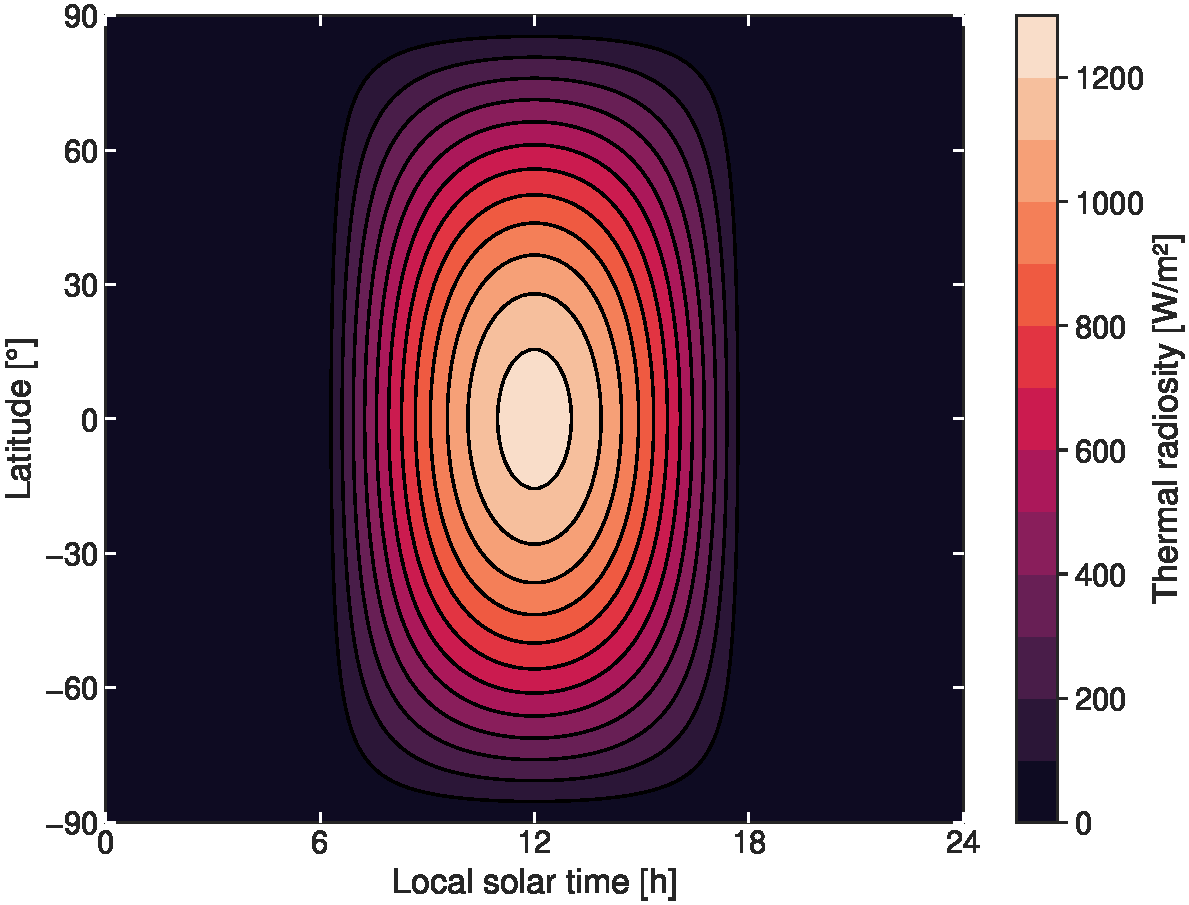
\includegraphics[width=\linewidth]{figures/plots/thermal_map.pdf}
    \caption{Map of lunar thermal emissions from the angle-based model (\cref{eq:radiosity-thermal-anglebased}). The emissivity is 0.95 and surface temperatures range between \qty{95}{\K} and \qty{385}{\K}, depending on the subsolar angle.}
    \label{fig:thermal-map}
\end{figure}

The thermal radiosity from the angle-based model with the aforementioned parameters is shown in \cref{fig:thermal-map}. The radiosity decreases with the cosine of the incidence angle and approaches negligible emissions of $J_\text{thermal} = \qty{6}{\irr}$ at nighttime. The maximum radiosity, which occurs below the subsolar point, is $J_\text{thermal} = \qty{1246}{\irr}$. This peak value agrees with the values used to design \gls{LRO}'s thermal control subsystem~\cite{Tooley2010}. The only effect that is not captured is the slow cooling by about \qty{25}{\L} between sunset and sunrise~\cite{Vasavada2012}, introducing a slight asymmetry; we use constant pre-sunrise temperatures throughout the night. We also do not model seasonal variations of surface temperature.






\subsection{Paneling of the Moon}

use 5 rings for moon due to convergence analysis and results from~\cite{Floberghagen1999}
\cite{Nicholson2010} also uses 5 rings for LRO
Need more with DLAM-1 than knocke due to higher frequency albedo dist or lower altitude?

show convergence plot
is within XX pct of 10 rings for 5 rings




\subsection{LRO target}

to find cannonball area and coefficient, some authors use raytracing~\cite{Hattori2019}, we just use weighted average
finding a single rp coefficien is virtually impossible since it changes~\cite[p~580]{Vallado2013}

Different values for A and Cr in literature:
\cite{Nicholson2010}: 14, 1.0 (for daily/not precision OD, no changing orientation, solar only) --> use this one
\cite{Bauer2016}: 10, 1.2 (no changing orientation, solar only)
\cite{Slojkowski2015}: first 1.67, then 0.96 after estimation
\cite{Mazarico2018}: 1.03 +- 0.24 (1.04 in sep, 1.4 in jun, but rather a scale factor for paneling than cannonball coefficient)

mass at start of science orbit (15 Sep 2009): 1271.9 kg
mass at end of science orbit (11 Dec 2011): 1087.0 kg
use end of science orbit mass for all scenarios to get worst case scenario
fixed mass to enable comparison
also show mass history

effect of self-shadowing on LRO orbit is small~\cite{Loecher2018}
neglecting self-shadowing overestimates area~\cite{Mazarico2009}, but minimal self-shadowing in most cases for LRO~\cite{Slojkowski2015}





\subsection{LRO orbit geometry}
% TODO check results quickly if we use both arcs

variation in altitude is in part due to assumption of spherical moon (polar radius is 2.1 km less than equatorial) -> leads to change in lunar RP magnitude over orbit
sun beta over year + eclipse periods

our maximum eclipse time of 48 min agrees with \cite{Tooley2010}

describe beta angle
maybe figure with orbit geometry for simulated arcs


\subsection{Simulation setup}

simulation setup in table, explanations in text

earth albedo + thermal radiation can be neglected for LRO since it is less than 0.1\% of solar radiation at moon

solar array tracks Sun, HGA tracks Earth~\cite{Tooley2010}
start at start at 26 June 2010 06:00:00
Earth eclipses Sun during this time
Moon does not eclipse Sun (Sun beta angle is about -90 deg, see~\cite{Tooley2010})

lunar eclipses avoided since we cannot represent multiple occultations

effects of neglecting terrain and self shadowing~\cite{Mazarico2018} sec 4.2 and 4.3


Operational LRO OD does not use lunar albedo due to computational demand, but used for offline reprocessing.
Self-shadowing from \citeauthor{Mazarico2009} is used for reprocessing~\cite{Nicholson2010}

arc length 2.5 days, which is also used for LRO orbit determination~\cite{Mazarico2011}
step 5 s, which is also used for LRO orbit determination~\cite{Mazarico2018}

MOON\_PA frame, IAU\_MOON is in worst case 155 m off~\cite{NAIF2020} (Special PCK and FK for Earth and Moon, slide 14)

integrator + propagator params



two arcs, one for beta = 0 and beta = 90
describe why These